\documentclass[aspectratio=169, 12pt]{beamer}

% --- Theme Setup ---
\usetheme{Madrid}
\usecolortheme{seahorse}
\setbeamertemplate{navigation symbols}{}
\setbeamertemplate{footline}[frame number]

% --- Packages ---
\usepackage{amsmath, amssymb}
\usepackage{graphicx}
\usepackage{booktabs}
\usepackage{xcolor}
\usepackage{listings}
\graphicspath{{../../plots/}}

% --- Custom Colors ---
\definecolor{topological}{HTML}{1f77b4}
\definecolor{highlight}{HTML}{2ca02c}
\definecolor{codebg}{HTML}{f5f5f5}

% --- Macros ---
\newcommand{\ket}[1]{|#1\rangle}
\newcommand{\bra}[1]{\langle#1|}

\title[Kitaev Chain — Block 3]{Majorana Modes in the Machine}
\subtitle{Week 5: Transitioning to Quantum Circuit Measurement}
\author{Dobromir Stoev \\ Edgar Harutyunyan \\ Guilherme Schewtschik \\ Jaskaran Singh \\ Zhengyi Liu \\ Zhenming Shi}
\institute{Advanced Seminar — AI-Augmented Theoretical Physics}
\date{\today}

\begin{document}

\begin{frame}
  \titlepage
\end{frame}

\begin{frame}{Week 5 Objectives: Moving to Block 3}
    \begin{itemize}
        \item \textbf{Main Goal:} Shift from "Exact Matrix Math" to "Gate-Based Simulation."
        \item \textbf{Task 1:} Ground State Preparation via VQE (Variational Quantum Eigensolver).
        \item \textbf{Task 2:} Defining the Non-local String Order Parameter $\mathcal{O}_{string}$.
        \item \textbf{Task 3:} Mapping Majorana Observables to Qubit Measurement Gates.
        \item \textbf{Task 4:} Numerical Evidence.
    \end{itemize}
\end{frame}

\begin{frame}{Task 1: VQE Circuit Ansatz (Visual)}
    \begin{columns}
        \column{0.5\textwidth}
        \textbf{Hardware-Efficient Ansatz:}
        \begin{itemize}
            \item Uses only $R_y$ to keep the state in the real domain.
            \item Linear CNOT entanglement mimics 1D hopping.
        \end{itemize}
        \column{0.5\textwidth}
        \centering
        \fbox{\begin{minipage}{0.9\textwidth}
            \centering
            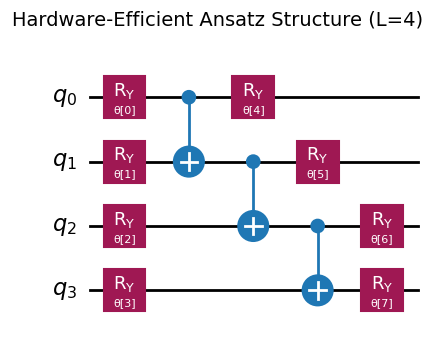
\includegraphics[width=\textwidth]{block3_VQE_Ansatz.png}
        \end{minipage}}
    \end{columns}
\end{frame}

\begin{frame}{$R_y$ Gate}
    For $L=4$, the configuration space consists of $2^4 = 16$ possible states:
    \[ \ket{\Psi} = c_0\ket{0000} + c_1\ket{0001} + \dots + c_{15}\ket{1111} \]
    \begin{block}{}
        Initially, $|\psi\rangle = [1, 0, 0, \dots, 0]^T$. An $R_y(\theta)$ gate on $q_0$ performs:
        \[ R_y(\theta)\ket{0} = \cos(\theta/2)\ket{0} + \sin(\theta/2)\ket{1} \]
        In the 16D vector, the value "1" splits:
        \begin{itemize}
            \item Index 0 ($\ket{0000}$): becomes $\cos(\theta/2)$
            \item Index 8 ($\ket{1000}$): becomes $\sin(\theta/2)$
        \end{itemize}
    \end{block}
\end{frame}


\begin{frame}{CNOT Gate}
    Entanglement occurs when a gate moves amplitudes between binary configurations.
    \begin{exampleblock}{CNOT(0,1) Operation}
        If $q_0$ is 1, flip $q_1$. In the vector:
        \begin{enumerate}
            \item $\ket{1000}$ (Index 9) satisfies the condition.
            \item It is transformed into $\ket{1100}$ (Index 13).
        \end{enumerate}
        Physical meaning: isolated excitations are combined into \textbf{paired states}, building the topological correlations needed for Majoranas.
    \end{exampleblock}
\end{frame}


\begin{frame}{Hilbert Space Evolution: Mathematical Verification}
    \textbf{Mathematical Constraint:} Post-entanglement states cannot be factored into independent single-qubit probabilities. The evolution must be tracked across the full $2^4 = 16$ dimensional state vector.
    
    \vspace{0.3cm}
    \textbf{State Vector Evolution Table (Tracking non-zero amplitudes):}
    
    \vspace{0.2cm}
    \begin{table}[h]
    \centering
    \renewcommand{\arraystretch}{1.5}
    \resizebox{\textwidth}{!}{
    \begin{tabular}{ccccc}
    \toprule
    \textbf{Index (Dec)} & \textbf{Basis ($q_0 q_1 q_2 q_3$)} & \textbf{Init State $|\psi_0\rangle$} & \textbf{Post $R_y(\theta_0)$ $|\psi_1\rangle$} & \textbf{Post CNOT$_{0 \to 1}$ $|\psi_2\rangle$} \\
    \midrule
    \textbf{0} & $|0000\rangle$ & $1$ & $\cos(\frac{\theta_0}{2})$ & $\cos(\frac{\theta_0}{2})$ \\
    1 & $|0001\rangle$ & $0$ & $0$ & $0$ \\
    \vdots & \vdots & \vdots & \vdots & \vdots \\
    \textbf{8} & $|1000\rangle$ & $0$ & $\sin(\frac{\theta_0}{2})$ & $\mathbf{0}$ \quad \textit{(Amplitude shifted)} \\
    \vdots & \vdots & \vdots & \vdots & \vdots \\
    \textbf{12} & $|1100\rangle$ & $0$ & $0$ & $\sin(\frac{\theta_0}{2})$ \\
    \vdots & \vdots & \vdots & \vdots & \vdots \\
    15 & $|1111\rangle$ & $0$ & $0$ & $0$ \\
    \bottomrule
    \end{tabular}
    }
    \end{table}

    \vspace{0.3cm}
    \textbf{Algebraic Operator Action:}
    \begin{itemize}
        \item \textbf{$R_y$ Tensor Product:} $\hat{U}_1 = R_y(\theta_0) \otimes I^{\otimes 3}$. Splits probability amplitude between index 0 and index 8.
        \item \textbf{CNOT Permutation Matrix:} $\hat{U}_2 = \text{CNOT}_{0\to 1} \otimes I^{\otimes 2}$. Executes conditional dimension shift: $\alpha|1000\rangle \xrightarrow{} \alpha|1100\rangle$.
    \end{itemize}
\end{frame}


\begin{frame}{Hamiltonian Simplification: The Pure YY Limit}
    \centering
    \fbox{\begin{minipage}{0.8\textwidth}
        \centering
        \textbf{General Qubit Mapping (Block 2):} \\
        $H_K = -\frac{\mu}{2}\sum Z_j + \frac{t-\Delta}{2}\sum X_j X_{j+1} + \frac{t+\Delta}{2}\sum Y_j Y_{j+1}$ \\
        \vspace{0.3cm}
        \textbf{Topological Sweet Spot ($t = \Delta$, $\mu = 0$):} \\
        $\mathbf{H = \sum_{j=0}^{L-2} Y_j Y_{j+1}}$
    \end{minipage}}
    \begin{itemize}
        \item \textbf{XX Cancellation:} Setting $t = \Delta$ (hopping = pairing) mathematically eliminates all $X_j X_{j+1}$ terms.
        \item \textbf{Field Removal:} Setting $\mu = 0$ removes the transverse $Z$ fields, reaching the deepest topological phase.
    \end{itemize}
\end{frame}


\begin{frame}{Numerical Verification: VQE Convergence Dynamics}
    \begin{columns}
        \column{0.55\textwidth}
        \centering
        \fbox{\begin{minipage}{0.95\textwidth}
            \centering
            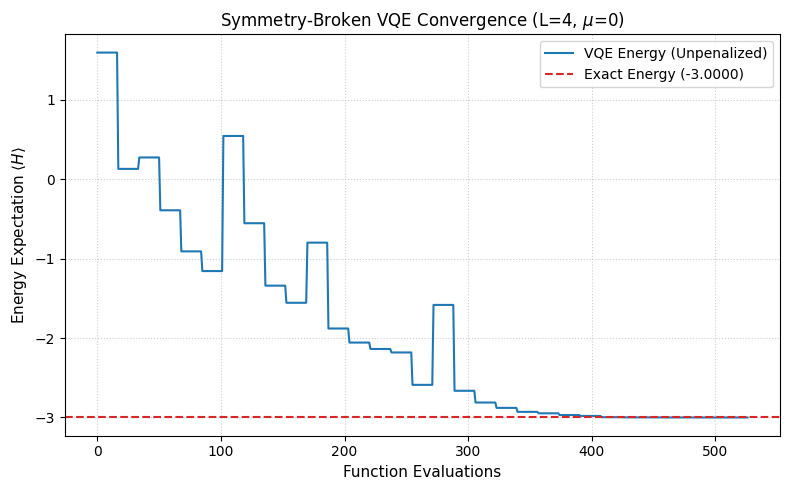
\includegraphics[width=\textwidth]{block3_VQE_Converage.png} 
        \end{minipage}}
        
        \column{0.45\textwidth}
        \textbf{Optimization Parameters:}
        \begin{itemize}
            \item \textbf{Algorithm:} L-BFGS-B (Gradient-based).
            \item \textbf{Cost Function:} $C(\vec{\theta}) = \langle H \rangle - \lambda \langle P \rangle$.
            \item \textbf{Penalty ($\lambda=0.1$):} Enforces strictly even parity ($P=+1$) selection, breaking topological degeneracy.
        \end{itemize}
        
    \end{columns}
\end{frame}



\begin{frame}{Task 2: String Operator}
    \centering
    \fbox{\begin{minipage}{0.9\textwidth}
        \centering
        \textbf{Boundary Majorana Correlator to Qubit Mapping:} \\
        \vspace{0.1cm}
        $\hat{O}_{corr} \propto i\gamma_{0,2}\gamma_{3,1} = i(Y_0)(Z_0 Z_1 Z_2 X_3) = -X_0 Z_1 Z_2 X_3$
    \end{minipage}}
    \vspace{0.15cm}
    \begin{itemize}
        \item \textbf{1. Breakdown of the Landau Paradigm:} The topological phase hosts no local symmetry breaking. All local single-qubit expectations strictly vanish:
        $$\forall j \in \{0,1,2,3\}, \quad \langle X_j \rangle = 0, \quad \langle Y_j \rangle = 0, \quad \langle Z_j \rangle = 0$$
        Non-local order parameters are mandatory to detect this hidden order.
        \item \textbf{2. Ground State Commutation Constraint:} A saturated non-zero invariant requires $[H, \hat{O}_{string}] = 0$. The naive boundary operator $\hat{O}_{naive} = X_0 X_3$ anti-commutes with $H$, creating high-energy quasiparticle excitations and yielding $\langle X_0 X_3 \rangle \equiv 0$.
    \end{itemize}
\end{frame}


\begin{frame}{Task 3: Measuring Topology via Basis Rotation}
    \centering
    \fbox{\begin{minipage}{0.6\textwidth}
        \centering
        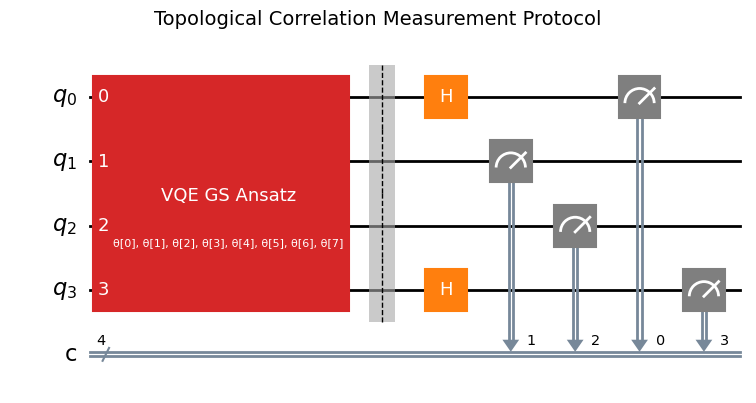
\includegraphics[width=0.8\textwidth]{block3_Measurement.png}
    \end{minipage}}
    
    Hardware measures in $Z$-basis. Majoranas live in $X$-basis.
    \begin{itemize}
        \item \textbf{Observable ($X_0Z_1Z_2X_3$)}
        \item \textbf{Hadamard ($H$) Gate:} Maps $X \to Z$.
        \item Applied to $q_0$ and $q_3$ to extract the non-local correlation.
    \end{itemize}
\end{frame}








\begin{frame}{Task 4: Numerical Evidence: The 1.0 Correlation}
    \centering
    \fbox{\begin{minipage}{0.6\textwidth}
        \centering
        \includegraphics[width=0.8\textwidth]{block3_Correlation.png}
    \end{minipage}}
    \begin{itemize}
        \item \textbf{Left ($Y_0$):} $\approx 0$ due to anti-commutation with the global parity operator ($\{Y_0, \hat{P}\} = 0$).
        \item \textbf{String ($X_0Z_1Z_2X_3$):} Exactly $1.0000$ (Theoretical limit).
        \item \textbf{Algebraic Symmetry:} The commutation $[H, \hat{O}_{corr}] = 0$ identifies this as a conserved topological invariant.
        \item \textbf{Result:} Non-local Topology confirmed in the gate-based model.
    \end{itemize}
\end{frame}



\begin{frame}{Summary \& Next Steps}
    \begin{itemize}
        \item \textbf{Completed:} VQE ground state preparation.
        \item \textbf{Discovery:} The non-local string order parameter is a robust topological signature.
        \item \textbf{Next:} Sweep $\mu$ to generate the full Phase Diagram using only quantum circuit results.
    \end{itemize}
\end{frame}

\end{document}
